\section*{06/09}

\underline{Алгоритм метода конечных элементов:}
\begin{enumerate}
	\item Дискретизация;
	\item Аппроксимация кусочно-непрерывными функциями;
	\item Решение СЛАУ.
\end{enumerate}
	
	\begin{center}
		\textbf{Дискретизация области}
	\end{center}

\begin{enumerate}
		\item Разделение тела на конечные элементы;
		\item Нумерация ($N$ узлов, $N$ элементов).
\end{enumerate}

\begin{figure}[h] 
	\begin{center}
		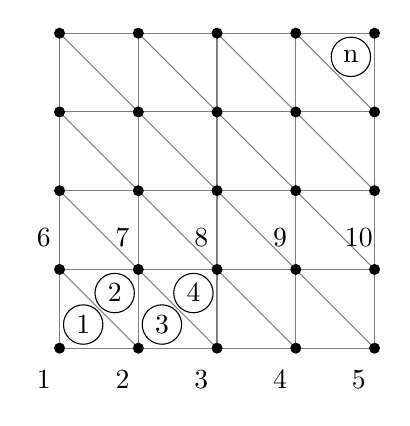
\begin{tikzpicture}
			\def\xmax{4}
			\def\ymax{4}
			
			\foreach \x in {0,1,...,\xmax} {
				\foreach \y in {0,1,...,\ymax} {
					\draw[gray] (\x, 0) -- (\x, \ymax);
					\draw[gray] (0, \y) -- (\xmax, \y);
				}
			}
			
			\foreach \x in {0,1,...,3} {
				\foreach \y in {0,1,...,3 } {
					\draw[gray] (\x, \y + 1) -- (\x + 1, \y);
				}
			}
			
			\foreach \x in {0,1,...,\xmax} {
				\foreach \y in {0,1,...,\ymax} {
					\fill (\x,\y) circle (2pt);
				}
			}
			
			\foreach \x in {1,2,...,5} {
				\node at (\x - 1.2, -0.4) {\x};
			}
			
			\foreach \x in {6,7,...,10} {
				\node at (\x - 6.2, 1.4) {\x};
			}
			
			\draw (0.3,0.3) circle (2.5mm); 
			\node at (0.3,0.3) {1}; 
			
			\draw (1.3,0.3) circle (2.5mm); 
			\node at (1.3,0.3) {3}; 
			
			\draw (0.7,0.7) circle (2.5mm); 
			\node at (0.7,0.7) {2}; 
			
			\draw (1.7,0.7) circle (2.5mm); 
			\node at (1.7,0.7) {4}; 
			
			\draw (3.7,3.7) circle (2.5mm); 
			\node at (3.7,3.7) {n}; 
			
		\end{tikzpicture}
	\end{center}
	\caption{Пример дискретизации области}
\end{figure}

\begin{figure}[h] 
	\begin{center}
		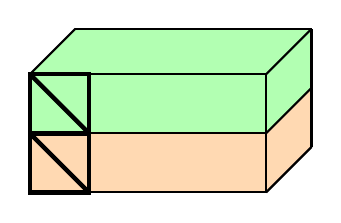
\begin{tikzpicture}[scale=1.5]
			\fill[orange!30] (0,0,1) -- (2,0,1) -- (2,0.5,1) -- (0,0.5,1) -- cycle;
			\fill[orange!30] (2,0,1) -- (2,0.5,1) -- (2,0.5,0) -- (2,0,0) -- cycle;
			
			\fill[green!30] (0,0.5,1) -- (2,0.5,1) -- (2,1,1) -- (0,1,1) -- cycle;
			\fill[green!30] (2,0.5,1) -- (2,1,1) -- (2,1,0) -- (2,0.5,0) -- cycle;
			\fill[green!30] (0,1,1) -- (2,1,1) -- (2,1,0) -- (0,1,0) -- cycle;
			
			
			\draw[thick] (0,0,1) -- (2,0,1) -- (2,1,1) -- (0,1,1) -- cycle; 
			
			\draw[thick] (2,0,0) -- (2,0,1); 
			\draw[thick] (2,1,0) -- (2,1,1); 
			\draw[thick] (0,1,0) -- (0,1,1); 
			\draw[thick] (2,0,0) -- (2,1,0); 
			\draw[thick] (0,1,0) -- (2,1,0); 
			
			\draw[thick] (0,0.5,1) -- (2,0.5,1); 
			\draw[thick] (2,0.5,0) -- (2,0.5,1);
			
			\draw[black, ultra thick] (0,0,1) rectangle (0.5,0.5,1);
			\draw[black, ultra thick] (0,0.5,1) rectangle (0.5,1,1);
			\draw[ultra thick] (0,0.5,1) -- (0.5,0,1);
			\draw[ultra thick] (0,1,1) -- (0.5,0.5,1);
			
			
		\end{tikzpicture}
	\end{center}
	\caption{Пример трехмерной области, состоящей из двух материалов}
\end{figure}

	\begin{figure}[H] 
	\begin{center}
		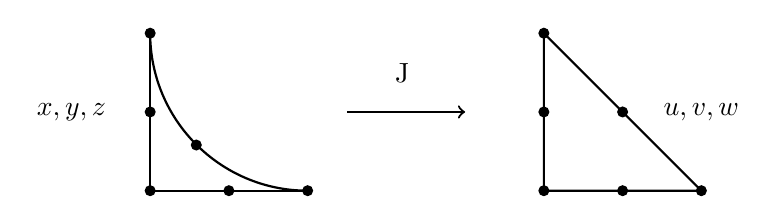
\begin{tikzpicture}
			
			\draw[thick] (0,0) arc[start angle=180, end angle=270, radius=2cm];
			\draw[thick] (2,-2) -- (0,-2);
			\draw[thick] (0,-2) -- (0,0);
			
			\draw[thick] (7,-2) -- (5,-2) -- (5,0)  -- cycle; 
			
			\draw[->, thick] (2.5,-1) -- (4,-1) ;
			\node at (3.2,-0.5) {J}; 
			
			\node at (-1,-1) {$x,y,z$};
			\node at (7,-1) {$u,v,w$};
			
			\fill (2,-2) circle (2pt);
			\fill (1,-2) circle (2pt);
			\fill (0,-2) circle (2pt);
			\fill (0,-1) circle (2pt);
			\fill (0,0) circle (2pt);
			\fill (0.58579, -1.42) circle (2pt);
			
			\fill (7,-2) circle (2pt);
			\fill (6,-2) circle (2pt);
			\fill (5,-2) circle (2pt);
			\fill (5,-1) circle (2pt);
			\fill (5,0) circle (2pt);
			\fill (6, -1) circle (2pt);
			
			
		\end{tikzpicture}
	\end{center}
	\caption{Приведение криволинейного элемента}
\end{figure}

\newpage
\underline{Замечания по разбиению:}
\begin{enumerate}
	\item Форма элемента должна быть близка к правильной;
	
\begin{figure}[h] 
	\begin{center}
		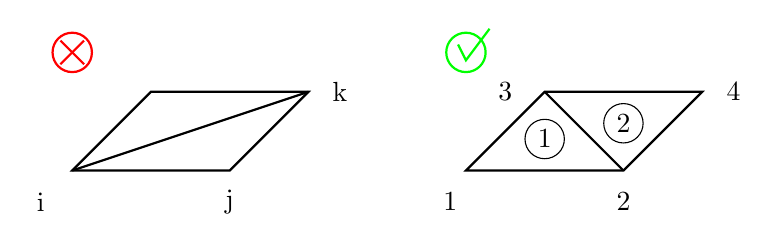
\begin{tikzpicture}
			
			\draw[thick] (0,0) -- (1,1) -- (3,1) -- (2,0)  -- cycle; 
			\draw[thick] (0,0) -- (3,1);
			
			\draw[thick] (5,0) -- (6,1) -- (8,1) -- (7,0)  -- cycle; 
			\draw[thick] (7,0) -- (6,1);
			
			\node at (-0.4,-0.4) {i};
			\node at (2,-0.4) {j};
			\node at (3.4,1) {k};
			
			\node at (4.8,-0.4) {1};
			\node at (7,-0.4) {2};
			\node at (5.5,1) {3};
			\node at (8.4,1) {4};
			
			\draw[red, thick] (0,1.5) circle (2.5mm);
			\draw[red, thick] (-0.15, 1.5-0.15) -- (0.15, 1.5+0.15);
			\draw[red, thick] (-0.15, 1.5+0.15) -- (0.15, 1.5-0.15);
			
			\draw[green, thick] (5,1.5) circle (2.5mm);
			\draw[green, thick] (4.9, 1.5+0.1) -- (5, 1.5-0.1) -- (5.3, 1.5+0.3);
			
			\draw (6,0.4) circle (2.5mm); 
			\node at (6,0.4) {1}; 
			
			\draw (7,0.6) circle (2.5mm); 
			\node at (7,0.6)  {2}; 
			
		\end{tikzpicture}
	\end{center}
	\caption{Пример плохой и хорошей дискретизации}
\end{figure}
	
	\item Все узлы конечного элемента должны совпадать.
	
	\begin{figure}[h] 
		\begin{center}
			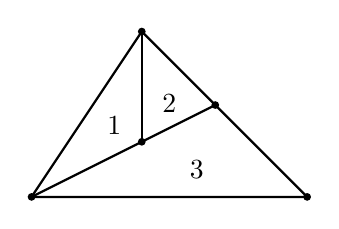
\begin{tikzpicture}[scale=0.7]
				
				\draw[thick] (0,0) -- (5,0) -- (2,3)  -- cycle; 
				\draw[thick] (0,0) -- (3.33333, 1.66667);
				\draw[thick] (2,3) -- (2,1);
				
				\fill (0,0) circle (2pt);
				\fill (5,0) circle (2pt);
				\fill (2,3) circle (2pt);
				\fill (3.33333, 1.66667) circle (2pt);
				\fill (2,1) circle (2pt);
				
				\node at (1.5,1.3) {1};
				\node at (2.5,1.7) {2};
				\node at (3,0.5) {3};
				
				
			\end{tikzpicture}
		\end{center}
		\caption{Пример плохой дискретизации}
	\end{figure}
	
\end{enumerate}

\underline{Замечание по нумерации узлов и конечных элементов:}

От нумерации узлов зависит ширина полосы ленты СЛАУ, поэтому узлы нужно нумеровать с короткой стороны для достижения наименьшей разницы между номерами узлов. Нумерация конечных элементов не важна, т.к. они привязаны к узлам.

\[
B=(R+1)\cdot Q
\]

где $B$ - ширина полосы ленты;

$R$ - максимальная по элементам величина наибольшей разности между узлами отдельного конечного элемента;

$Q$ - кол-во степенй свободы (число неизвестных).

\newpage
\underline{Нумерация треугольников против ЧС, начало с отдельных узлов.}
\begin{figure}[h] 
	\begin{center}
		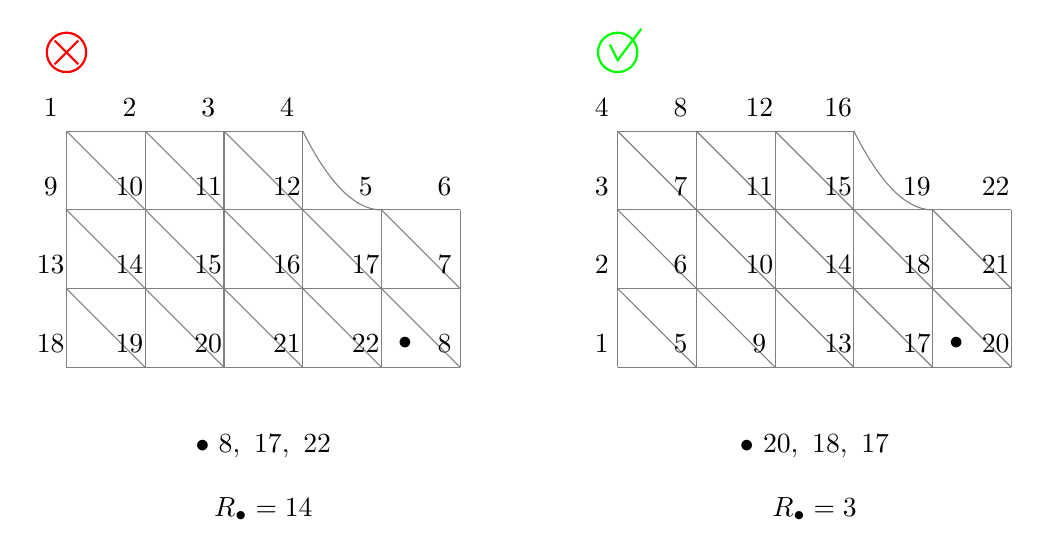
\begin{tikzpicture}[domain = -1:0] 
			\foreach \x in {0,1,...,3} {
				\foreach \y in {0,1,...,3} {
					\draw[gray] (\x, 0) -- (\x, 3);
					\draw[gray] (0, \y) -- (3, \y);
				}
			}
			
			\foreach \x in {0,1,...,2} {
				\foreach \y in {0,1,...,2 } {
					\draw[gray] (\x, \y + 1) -- (\x + 1, \y);
				}
			}
			
			\foreach \x in {0,1,...,2} {
				\foreach \y in {0,1,...,2} {
					\draw[gray] (\x+3, 0) -- (\x+3, 2);
					\draw[gray] (3, \y) -- (5, \y);
				}
			}
			
			\foreach \x in {0,1} {
				\foreach \y in {0,1} {
					\draw[gray] (\x+3, \y + 1) -- (\x + 4, \y);
				}
			}
			
			\draw[gray] plot (\x+4, \x * \x+2);
			
			\foreach \x in {1,2,...,4} {
				\node at (\x - 1.2, 3.3) {\x};
			}
			
			\foreach \x in {9,10,...,12} {
				\node at (\x - 9.2, 2.3) {\x};
			}
			
			\foreach \x in {13,14,...,17} {
				\node at (\x - 13.2, 1.3) {\x};
			}
			
			\foreach \x in {18,19,...,22} {
				\node at (\x - 18.2, 0.3) {\x};
			}
			
			\node at (3.8, 2.3) {5};
			
			\foreach \x in {6,7,...,8} {
				\node at (4.8, 8.3 - \x) {\x};
			}
			
			\node at (4.3, 0.3) {$\bullet$};
			\node at (2.5,-1) {$\bullet\ 8,\ 17,\ 22$};
			\node at (2.5,-1.8) {$R_\bullet = 14$};
			
			%second pic
			\foreach \x in {7,8,...,10} {
				\foreach \y in {0,1,...,3} {
					\draw[gray] (\x, 0) -- (\x, 3);
					\draw[gray] (7, \y) -- (10, \y);
				}
			}
			
			\foreach \x in {0,1,...,2} {
				\foreach \y in {0,1,...,2 } {
					\draw[gray] (\x+7, \y + 1) -- (\x + 8, \y);
				}
			}
			
			\foreach \x in {7,8,...,9} {
				\foreach \y in {0,1,...,2} {
					\draw[gray] (\x+3, 0) -- (\x+3, 2);
					\draw[gray] (10, \y) -- (12, \y);
				}
			}
			
			\foreach \x in {0,1} {
				\foreach \y in {0,1} {
					\draw[gray] (\x+10, \y + 1) -- (\x + 11, \y);
				}
			}
			
			\draw[gray] plot (\x+11, \x * \x+2);
			
			\foreach \x in {1,2,...,4} {
				\node at (6.8, -0.7+\x) {\x};
			}
			
			\foreach \x in {5,6,...,8} {
				\node at (7.8, -4.7+\x) {\x};
			}
			
			\foreach \x in {9,10,...,12} {
				\node at (8.8, -8.7+\x) {\x};
			}
			
			\foreach \x in {13,14,...,16} {
				\node at (9.8, -12.7+\x) {\x};
			}
			
			\foreach \x in {17,18,...,19} {
				\node at (10.8, -16.7+\x) {\x};
			}
			
			\foreach \x in {20,21,...,22} {
				\node at (11.8, -19.7+\x) {\x};
			}
			
			\node at (11.3, 0.3) {$\bullet$};
			\node at (9.5,-1) {$\bullet\ 20,\ 18,\ 17$};
			\node at (9.5,-1.8) {$R_\bullet = 3$};
			
			
			\draw[red, thick] (0,4) circle (2.5mm);
			\draw[red, thick] (-0.15, 4-0.15) -- (0.15, 4+0.15);
			\draw[red, thick] (-0.15, 4+0.15) -- (0.15, 4-0.15);
			
			\draw[green, thick] (7,4) circle (2.5mm);
			\draw[green, thick] (6.9, 4+0.1) -- (7, 4-0.1) -- (7.3, 4+0.3);
			
			
		\end{tikzpicture}
	\end{center}
	\caption{Пример правильной и неправильной нумерации узлов}
\end{figure}



Форма записи КЭ в файл(трехмерный случай):
\[
	\begin{rcases*}
		\begin{matrix}
			1 & x_1 & y_1 & z_1 \\
			2 & x_2 & y_2 & z_2 \\
			\cdots & \cdots & \cdots & \cdots\\
			n & x_n & y_n & z_n \\
		\end{matrix}
	\end{rcases*}
	\text{номера узлов и их координаты} 
\]

\[	
	\begin{rcases*}
		\begin{matrix}
			\textcircled{1} & 1 & 2 & 3 \\
			\textcircled{2} & 4 & 3 & 2 \\
			\cdots & \cdots & \cdots & \cdots\\
			\textcircled{n} & \cdots & \cdots & \cdots\\
		\end{matrix}
	\end{rcases*}
	\begin{matrix}
		\text{номера КЭ и номера узлов, из}  \\
		\text{которых они состоят}
	\end{matrix}	
\] 
\newpage
\indent \underline{Замечания о порядке узлов, составляющих КЭ:} 
\begin{enumerate}
	\item Обход узлов КЭ принято делать против часовой стрелки (для того, чтобы нормали были направлены в одну сторону); 
	\item Нумерацию желательно делать таким образом, чтобы соответствующие узлы попали в одно и то же место СЛАУ. 
\end{enumerate} 

\indent Пояснение к замечанию 2: \\
\indent Обратимся к Рисунку 4. Представим, что мы накладываем один КЭ на другой. Первый КЭ начнем нумеровать с узла №1 --- (1-2-3), тогда второй КЭ начнем обходить с узла №4 --- (4-3-2) и тд.
